\documentclass[12pt]{article}
\usepackage{amsmath, graphicx, caption,array, amsthm}
\usepackage{amsfonts, xcolor, physics, listings,verbatim}
\usepackage{amssymb,empheq, mathrsfs, comment, subfig, hyperref, url, fancyhdr, tikz, booktabs, geometry, enumitem, textcomp, subfig}
\usepackage[T1]{fontenc} % for \symbol{92} 
% Command "alignedbox{}{}" for a box within an align environment
% Source: http://www.latex-community.org/forum/viewtopic.php?f=46&t=8144
\newlength\dlf  % Define a new measure, dlf
\newcommand\alignedbox[2]{
% Argument #1 = before & if there were no box (lhs)
% Argument #2 = after & if there were no box (rhs)
&  % Alignment sign of the line
{
\settowidth\dlf{$\displaystyle #1$}  
    % The width of \dlf is the width of the lhs, with a displaystyle font
\addtolength\dlf{\fboxsep+\fboxrule}  
    % Add to it the distance to the box, and the width of the line of the box
\hspace{-\dlf}  
    % Move everything dlf units to the left, so that & #1 #2 is aligned under #1 & #2
\boxed{#1 #2}
    % Put a box around lhs and rhs
}
}

\addtolength{\oddsidemargin}{-1in}
\addtolength{\evensidemargin}{-1in}
\addtolength{\textwidth}{1.75in}
\addtolength{\topmargin}{-1in}
\addtolength{\textheight}{1.75in}
\newcommand{\contra}{$\rightarrow\leftarrow$}
\newcommand{\tb}{  \textbackslash  }
\newcommand{\bj}{\ \Longleftrightarrow \ }

%bailey meche
\begin{document}
%bailey meche
	\begin{center}
		ECMA 33230: Macroeconomic Crises - Spring 2025\\
        Problem Set 2: The Credit Crunch \\
		Due Date: April 28, 2025 \\
        Bailey Meche
	\end{center}

\begin{enumerate}
        \item (4 points) Describe the significance of limited commitment and limited enforcement for sovereign default. What types of costs are typically observed in the aftermath of a default event?
    \subsubsection*{Solution}

    In sovereign default models, limited commitment refers to the decision of the government to repay debt back to creditors based solely on their relative utility. Limited enforcement refers to the few external forces to incentivize repayment by the government to its creditors in the case where it may be more profitable for it to default. In the discussed models, the only enforcement tools offered are reputation loss by financial exclusion and economic damage via output loss. These are often not enough to completely disincentivize default, hence there exists a limited enforcement problem. 

    
    \item (12 points) {Eaton-Gersovitz (1981) model:} A country issues debt $b' > 0$ at a price $q(b')$ in period 1 to roll over outstanding debt $b > 0$. The benevolent and strategic government lacks commitment as to whether it repays or defaults on its debt in period 2. Output in period 2 is stochastic and denoted by $y'(s) = \sqrt{s}$, where each realization of the state $s \in \{1, 4, 9\}$ occurs with probabilities:
    \[
    P(s=1) = 0.2, \quad P(s=4) = 0.2, \quad P(s=9) = 0.6.
    \]
    Default entails a proportional output loss of a fraction $\kappa = 0.2$ and is preferred when it delivers a higher utility of consumption $u(c) = \log(c)$ in the second period. Risk-neutral competitive lenders face a risk-free net interest rate $r = 0.2$.

    \begin{enumerate}[label=(\alph*)]
        \item (4 points) What is the maximum default probability and the maximum debt the government can issue at which the sovereign net interest rate stays at or below 50\%?
        \subsubsection*{Solution}

        Setting up this model, we have 
        \begin{itemize}
            \item $t=1: \ $ country sells bonds $b'$ at a price $q$ to lenders with outstanding debt 
            \[ b = q(b') \cdot b' > 0\]
            \item $t=2: \ $ government decides to repay 1 dollar per bond or default with output 
            \[ y'(s) = \begin{cases}
                y'(s) & \text{repay}
                \\ (1-\kappa)y'(s) & \text{default}
            \end{cases} = \begin{cases}
                \sqrt{s} & \text{repay}
                \\ 0.8\sqrt{s}  & \text{default}
            \end{cases} \quad  \text{ for } s \in \{1, 4, 9\}.
            \]
        \end{itemize}
        Government problem: 
        \begin{align*}
            \max_{b'}& \mathbb{E}_s \left\{ \max \left\{ V^r(b',s) , \ V^d(s)  \right\}  \right\} & s.t. &  &b=q(b')\cdot b' 
            \\ =\max_{b'}& \mathbb{E}_s \left\{ \max \left\{u(y'(s) - b') , \ u((1-\kappa)y'(s))  \right\}  \right\}
            \\ =\max_{b'}& \mathbb{E}_s \left\{ \max \left\{\log(\sqrt{s} - b') , \ \log(0.8\sqrt{s})  \right\}  \right\}
        \end{align*}
        Lender's problem: (risk-neutral and competitive)
        \begin{align*}
            \max_{b'}& -q\cdot b' + \Pr(\text{repay}) \cdot \frac{b'}{1+r}
        \end{align*}
        which provides the debt price schedule 
        \begin{align}
            q(b') &= \frac{\Pr\left( u(y'(s) - b') \geq u((1-\kappa)y'(s)) \right)}{1+r}\notag 
            \\ &= \frac{\Pr\left( \log(\sqrt{s} - b') \geq \log(0.8\sqrt{s})   \right)}{1.2}. \label{2a}
        \end{align}

        To find the maximum default probability  at which the sovereign net interest rate stays at or below 50\%, we use the debt price schedule whereby 
         \begin{align*}
              \frac{1}{q(b')}-1 &\leq 0.5
              \\ \frac{1.2}{1-\Pr(\text{default})} -1&\leq 0.5
              \\ 1-\Pr(\text{default})&\leq 0.8
         \end{align*}
        Hence, the maximum default probability with these conditions is 20\%.      
        
        To find the maximum debt the government can issue at which the sovereign net interest rate stays at or below 50\%, we solve for $\Pr$(default) as a function of $b'$ before using \eqref{2a} to solve for probability:
        \begin{align}
            D(b',s) = \ V^r(b',s) &< V^d(s)\notag
            \\ u(y'(s) - b') &< u((1-\kappa)y'(s))\notag
            \\ \sqrt{s} - b' &< 0.8\sqrt{s}\notag
            \\ b' &> 0.2\sqrt{s}\notag
            \\ D(b',s) &= \begin{cases}
                b' > 0.2 & s=1
                \\ b' > 0.4& s=4
                \\ b' > 0.6& s=9
            \end{cases} \notag
            \\ \Pr(\text{default}) &= \begin{cases}
                0 & b' \leq 0.2
                \\ 0.2 & 0.4 \geq b' > 0.2 
                \\ 0.6 &0.6 \geq b' > 0.4
                \\ 1 & b' > 0.6
            \end{cases} \label{2b_d}
            \\ \Pr(\text{repay}) &= \begin{cases}
                1 & b' \leq 0.2
                \\ 0.8 & 0.4 \geq b' > 0.2 
                \\ 0.4 &0.6 \geq b' > 0.4
                \\ 0 & b' > 0.6
            \end{cases}\label{2b_r}
        \end{align}
        So, the maximum debt $b'$  the government can issue at which the sovereign net interest rate stays at or below 50\%, which we know to be where $\Pr(\text{default})\leq 0.2$, is using \eqref{2b_d}:
        \[ \arg\max \{\Pr(\text{default})\leq 0.2\}= \boxed{b' = 0.4}.\]

        \item (3 points) What is the maximum debt the government can issue at which the sovereign spread stays zero?
        \subsubsection*{Solution}

        The sovereign debt function is given as a function of \eqref{2a}
        \begin{align*}
            r^s &= \frac{1}{q(b')} - (1+r) 
            \\ &= \frac{1.2}{\Pr\left( \log(\sqrt{s} - b') \geq \log(0.8\sqrt{s})   \right)} - 1.2
        \end{align*}
        Solving for the maximum debt the government can issue at which the sovereign spread stays zero, set
        \begin{align*}
            \frac{1.2}{\Pr\left( \log(\sqrt{s} - b') \geq \log(0.8\sqrt{s})   \right)} - 1.2 &= 0
            \\ \Pr\left( \log(\sqrt{s} - b') \geq \log(0.8\sqrt{s})   \right) &= 1
        \end{align*}
        Solving for $b'$ using \eqref{2b_r}, we have 
        \[ \arg\max \{\Pr(\text{repay})=1\}= \boxed{b' = 0.2}.\]
        
        \item (5 points) Imagine the outstanding debt is $b = 0.22$. How much debt does the government issue to exactly roll it over? What is the sovereign gross interest rate?
        \subsubsection*{Solution}

        Using the $(b' \times  q(b')b')$ Laffer curve (Figure \eqref{fig:2c}) and the roll-over constraint for this model, we have the intersection for this level $b = 0.22$ at $b' = 0.33.$ Hence,  the government issue to exactly $b' = 0.33$ at $q(b') = \frac{2}{3}$ and the sovereign gross interest rate $\frac{3}{2}$, or 50\%.
        \begin{figure}[h]
            \centering
                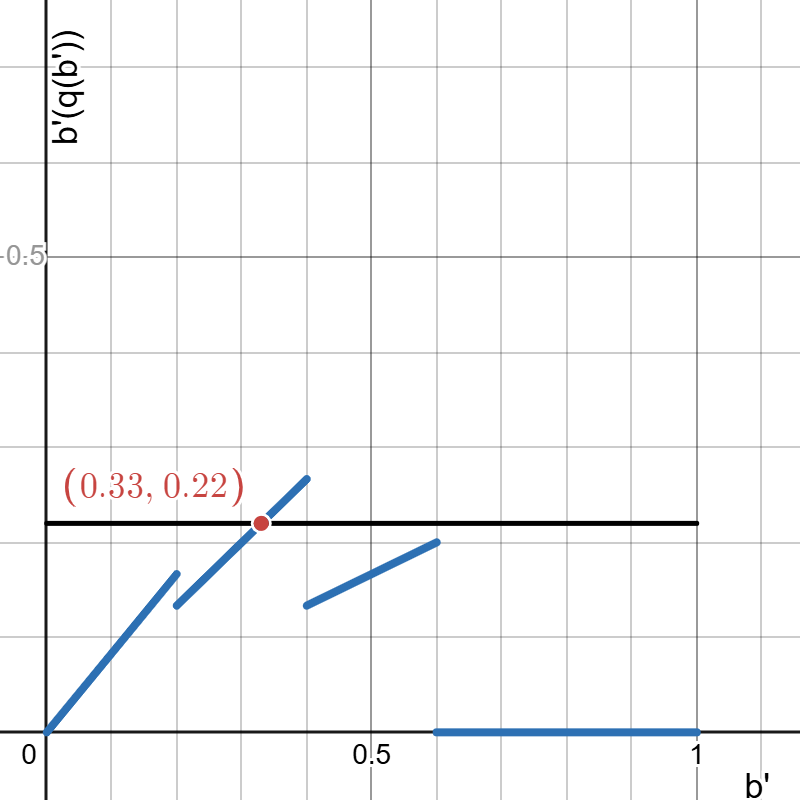
\includegraphics[width=0.5\textwidth]{pset2/2c_latter_curve.png}
                \caption{Laffer Curve}
                \label{fig:2c}
        \end{figure}
        
    \end{enumerate}

    \item (14 points) {Arellano (2008) model:} The benevolent and strategic government of a small open economy maximizes an expected infinite stream of period utilities from consumption $u(c)$, discounted with a discount factor $\beta$. Stochastic endowments $y \in \{2, 2.5, 3\}$ follow a Markov process with the transition matrix:

    \[
    P = \begin{pmatrix}
    p_{11} & p_{12} & p_{13} \\
    p_{21} & p_{22} & p_{23} \\
    p_{31} & p_{32} & p_{33} \\
    \end{pmatrix}
    = \begin{pmatrix}
    0.8 & 0.2 & 0.0 \\
    0.2 & 0.6 & 0.2 \\
    0.05 & 0.25 & 0.7 \\
    \end{pmatrix}
    \]

    where each entry $p_{ij}$ denotes the transition probability $\Pr(y' = y_j | y = y_i)$. The sovereign sells bonds $B'$ ($B' < 0$ means debt) facing a pricing function $q(B', y)$ to risk-neutral lenders. Lenders are competitive and take the default probability $\delta$ as given, stemming from the government’s limited commitment to debt repayment. The international risk-free net interest rate is $r = 0.017$. Default entails an output loss $h(y) \leq y$ and a stochastic exclusion from credit markets with probability $(1 - \theta)$. Let $V^o(B, y)$ be the value of integration, $V^r(B, y)$ be the value of repayment and $V^d(y)$ be the value of default. Assume that the value functions that solve the model can be represented as follows:

    \[
    V^r(B, y) = 0.6B + 0.3y^2, \quad V^d(y) = 0.2y
    \]

    \begin{enumerate}[label=(\alph*)]
        \item (5 points) Set up the lender’s problem and derive the first-order condition. Then write down the equilibrium pricing function and explain why the pricing schedule is a function of $B'$ and $y$.
        \subsubsection*{Solution}
        
        In this model, we have a representative household with preferences 
        \[ \mathbb{E}_0 \sum_{t=0}^\infty \beta^t \mu(c_t),\]
        stochastic income $y_t\in Y$ following a Markov process with transition probabilities given in the matrix $P$. The risk-neutral, foreign, competitive lenders need to break even in expected value. They have the problem 
        \begin{align*}
            \max_{B_{t+1}} q_t B_{t+1} - \frac{(1-\delta_t)B_{t+1}}{1+r}
        \end{align*}
        which provides the equilibrium pricing function (debt price schedule) as a function of $B'$ and $y$:
        \[ q(B_{t+1}, y_t) = \frac{1-\delta(B_{t+1}, y_t)}{1+r}\] where $\delta\bigl(B',y\bigr)= \Pr\bigl(\text{default in }t+1\mid B_{t+1}=B',\,y_t=y\bigr).$
        We have $q(B_{t+1}, y_t), \delta(B_{t+1}, y_t)$ in this pricing function because the larger the debt \(B'\) you promise to repay tomorrow, the more tempted the government will be to default once it observes its actual output.  A higher \(B'\) therefore mechanically raises \(\delta(B',y)\), which pushes down the price \(q\). Concerning dependence on $y$, if today’s income \(y\) is low, then even a modest \(B'\) may look hard to service; conversely, if \(y\) is high, the government can safely take on more debt before default becomes attractive.  Thus the mapping \(B'\mapsto\delta(B',y)\) shifts with \(y\), and so does the price \(q(B',y)\).
        

        \item (2 points) What is the range of the debt price? What is the range of the sovereign spread?
        \subsubsection*{Solution}
        The range of the debt price is  \[ q(B_{t+1}, y_t) \in \left[ 0, \frac{1}{1+r}\right] = \left[0,\frac{1}{1+0.017}\right] =\left[0,0.983\right].\] %\frac{1000}{1017}
        The range of the sovereign spread is 
        \[ r^s \in \left[ -(1+r), \frac{1}{1+r} -(1+r)\right] =\left[-1.017, -0.0337\right] .\] %  -\frac{1017}{1000}, -\frac{34289}{1017000}
        

        \item (4 points) What are the repayment and default sets for $B = -1.5$ and $B = -2.3$?
        \subsubsection*{Solution}

        For the solved value functions $V^r(B, y) = 0.6B + 0.3y^2, \ V^d(y) = 0.2y$, we have
        \begin{align*}
            A(B=-1.5) &= \{ y \in Y: \ V^r(B,y) \geq V^d(y) \} 
            \\ &=  \{ y \in Y: \ 0.6(-1.5) + 0.3y^2 \geq 0.2y \} 
            \\ &= \{ y \in Y: y\leq -1.4305,\  y \geq 2.097 \} 
            \\ &= \{ 2.5, 3\}
            \\ D(B=-1.5) &= \{ y \in Y: \ V^r(B,y) < V^d(y) \} 
            \\ &= \{ y \in Y: -1.4305 <  y < 2.097 \} 
            \\ &= \{2\}
            \\ A(B=-2.3) &= \{ y \in Y: \ 0.6(-2.3) + 0.3y^2 \geq 0.2y \} 
            \\ &= \{ y \in Y: y\leq -1.837,\  y \geq 2.5038 \} 
            \\ &= \{3\}
             \\ D(B=-2.3) &= \{ y \in Y: \ V^r(B,y) < V^d(y) \} 
            \\ &= \{ y \in Y: -1.837<  y < 2.5038 \} 
            \\ &= \{ 2,2.5\}
        \end{align*}

        \item (3 points) Calculate the default probabilities $\delta(B', y)$ for each current endowment state given that the government issues $B' = -1.5$.
        \subsubsection*{Solution}

        Define the default set: 
        \begin{align*}
            D(B') &= \{ y \in Y: \ V^r(B',y) < V^d(y) \} 
            \\ D(B'=-1.5) &= \{ y \in Y: -1.4305 <  y < 2.097 \}
            = \{ 2\}
        \end{align*}
         so we have 
        \begin{align*}
            \delta(B'= -1.5, y) &= \sum_{D(B'= -1.5)} \Pr(y'|y)
            \\ &=\Pr(y'=2|y)
       \\ & = \begin{cases}
            0.8& y=2
            \\ 0.2 & y=2.5
            \\ 0.02 & y=3
        \end{cases}
        \end{align*}

    \end{enumerate}

    \item (12 points) Consider the Arellano (2008) model of sovereign default discussed in class. Sketch a 2-D graph that displays the default policy of the government in terms of the default income threshold $y^*(B)$. Your graph should include at least the following description/labels as defined in the lecture: $y^*(B)$, 0, $y$, $B$, $\bar{B}$, $\underline{B}$, $y_{\min}$, $y_{\max}$, $B^*$, $Z$, repayment region, default region.
    \subsubsection*{Solution}

    We plot a $(B \times y)$ figure for the following function $y^*: \mathbb{R}^{\leq 0} \to \mathbb{R}^{\geq 0}$:
\begin{align*}
  V^r(B,y) &= 2B + y^2 
  \\ V^d(y) &= 0.3y
  \\ y^*(B) &= \frac{1}{2}\left(0.3+\sqrt{(-0.3)^{2}-4\left(2B\right)}\right).
\end{align*}
    See Figure \eqref{fig:4} for this plot.
    \begin{figure}[h]
            \centering
                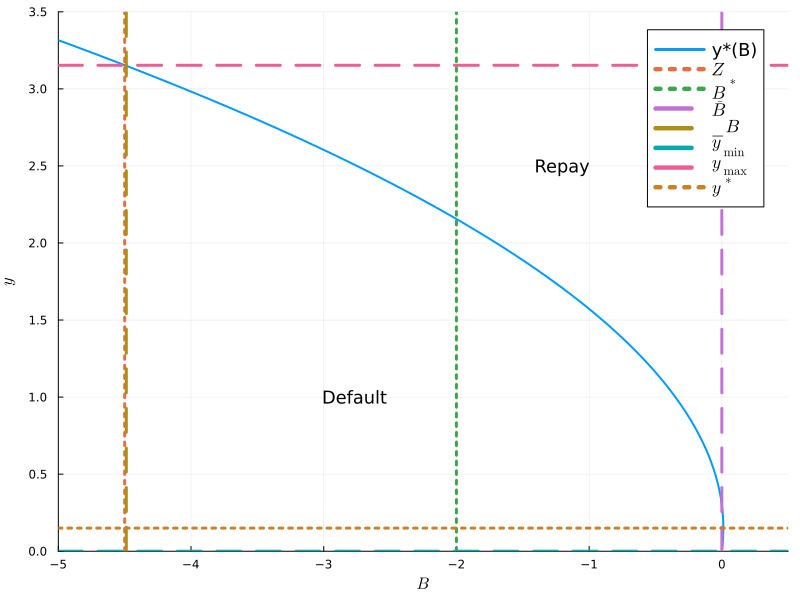
\includegraphics[width=0.65\textwidth]{pset2/q4.png}
                \caption{Arellano (2008) - Problem 4}
                \label{fig:4}
        \end{figure}

    \newpage 
    \item (20 points) The benevolent and strategic government of a small open economy maximizes an expected infinite stream of period utilities from consumption $u(c)$, discounted with a discount factor $\beta = 0.8$. Stochastic endowments $y_t \geq 0$ follow a Markov process with the AR(1) transition rule:
    \[
    f(y_{t+1} \mid y_t): \quad \ln(y_{t+1}) = \rho \ln(y_t) + \sigma_\varepsilon \varepsilon_{t+1},
    \]
    where $\rho = 0.9$ is the persistence and $\sigma_\varepsilon = 0.5$ scales the standard deviation of innovations $\varepsilon_t$, which are drawn from a uniform distribution $U[0, 1]$. The sovereign sells bonds $B'$ ($B' < 0$ means debt) facing a pricing function $q(B', y)$ to risk-neutral lenders. Lenders are competitive and take the default probability $\delta$ as given. The international risk-free net interest rate is $r = 0.01$. Default entails an output loss $c(y) \leq y$ and a stochastic exclusion from credit markets with probability $(1 - \theta)$, where $\theta = 0.2$. During exclusion, previous debt is frozen and no new debt can be issued. Upon reintegration, the government imposes a haircut $h = 0.7$ on the frozen debt, meaning it has now outstanding debt of a share $1 - h$ of previous debt. 

    \textit{Hint: Recall that the pdf and cdf of a uniform distribution are closed form.}

    \begin{enumerate}%[label=(\alph*)]
        \item (5 points) Set up the recursive formulation of the government’s problem.
        \subsubsection*{Solution}

        For endowment in $t=1$ as $y$, consumption $c(y)$, and state $s\in \{$repay, default\}, the government's budget constraint is given by:
        \[ c(y,s) = \begin{cases}
            y + B - q(B',y)B' & s=\text{repay}
            \\ hy & s=\text{default}
        \end{cases} 
        \]
        At the beginning of each period, the government inherits $B<0$ and observes $y$ based on $(B,y)$ decides to repay or default. The value function of the government deciding to repay or default is given by 
        \begin{align*}
            V^o(B,y) &= \max \{V^r(B,y), V^d(y)\}
            \\ V^r(B,y) &= \max_{B' \geq -Z} \left\{u(c(y,s=\text{repay}))+ \beta \int_{y'}  V^o(B',y') f(y' \mid y)dy' \right\}
            \\&= \max_{B' \geq -Z} \left\{u(y + B - q(B',y)B')+ \beta \mathbb{E}_{y'} \left[  V^o(B',y') \mid y  \right]\right\}
            \\ V^d(y) &=  u(c(y,s=\text{default})) + \beta \int_{y'}  \left[ (1-\theta)V^d(y') + \theta V^o(0,y') \right] f(y' \mid y) dy'
            \\ &=  u(hy) + \beta\mathbb{E}_{y'}  \left[ (1-\theta)V^d(y') + \theta V^o(0,y') \right] .
        \end{align*}

        \item (4 points) Suppose the default threshold $y^*(B)$, at which the government is indifferent between default and repayment in the $(B, y)$-space, is given by $y^*(B) = 5 + \frac{15}{B - 3}$. What is the default probability if the government chooses $B' = -1$ and is currently in state $y = 1.1$?
        \subsubsection*{Solution}

        The given threshhold $y^*(B)$ indicates that the government chooses to default if 
        \[ y' < y^*(B' = -1) = 5 + \frac{15}{B' - 3}= 1.25.\]
        We can find  the default probability given  $y = 1.1$ by computing 
        \begin{align*}
            \delta(B',y) &= \int_{D(B')} P(y'|y)dy'
            = \int^{y^*(B')}_{e^{\rho\ln(y)}} \frac{2}{y'}dy'
            = \int^{1.25}_{1.0896} \frac{2}{y'}dy'
            \approx 0.275.
        \end{align*}

        \item (5 points) As before, $y^*(B) = 5 + \frac{15}{B - 3}$, but suppose the endowment level is $y = 1$ today. Calculate the thresholds $\bar{B}$ and $\underline{B}$ for $B'$, where the default set will be either empty or comprise all endowment levels, respectively.
        \subsubsection*{Solution}

        Given that  the endowment level is $y = 1$ today, we the range for $y$ values 
        \begin{align*}
            f(y' \mid y = 1): \quad  \ln(y') &= \rho \ln(1) + \sigma_\varepsilon \varepsilon'
            \\ y'&= e^{\rho \ln(1) + \sigma_\varepsilon \varepsilon'}
        \end{align*}
        so we have $y' \sim U[1,1.6487]$.
        \begin{align*}
        D(B) &= \left\{ y' \geq 0 : \ y' < 5 + \frac{15}{B - 3} \right\}
           \\  \bar{B} &= \inf \{ B: \  D(B)=\emptyset\} 
           &= \inf\left\{ B: \ 5+\frac{15}{B-3} = \min y' \right\}
           = \{ -0.75\} 
\\            \underline{B} &= \sup \{ B: \  D(B)=y\} 
             &=  \sup\left\{ B: \ 5+\frac{15}{B-3} = \max y'  \right\} = \{ -1.4759\} 
        \end{align*}

        \item (6 points) As before, $y^*(B) = 5 + \frac{15}{B - 3}$ and $y = 1$. Plot today’s Laffer curve in Julia. Plot $B'$ on the x-axis from -2 to 0.5. Include your code.
        \subsubsection*{Solution}

        See Figure \eqref{fig:5} for this plot.
    \begin{figure}[h]
            \centering
                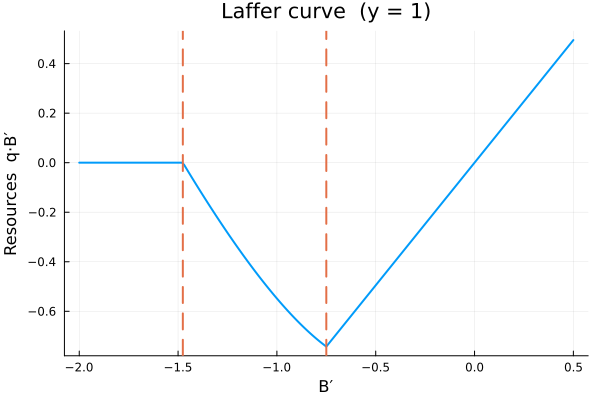
\includegraphics[width=0.6\textwidth]{pset2/q5.png}
                \caption{Laffer curve - Problem 5}
                \label{fig:5}
        \end{figure}

        
    \end{enumerate}

        \item (8 points) Suppose a country has debt of face value 150 billion USD. Without any intervention the probability of default is 0.75, in which case there is a $2/3$ haircut on the debt and creditors will only receive one third of the face value.

    \begin{enumerate}%[label=(\alph*)]
        \item (2 points) What is the expected repayment value without intervention? What is the secondary market price of the debt?
        \subsubsection*{Solution}

        In USD (billions):
        \begin{align*}
            \text{ expected repayment value} &= (0.25) \cdot 150 + (0.75) \cdot \left( \frac{1}{3} \cdot 150\right) &= 75
            \\ \text{secondary market price of the debt} &= \frac{\text{ expected repayment value}}{\text{face value}} = \frac{75}{150} = 0.5
        \end{align*}

        \item (2 points) How much do creditors gain or lose if they forgive 30 billion USD?
        \subsubsection*{Solution}

        \begin{align*}
            & \underline{\text{Initial}} & \underline{\text{after debt forgiveness}}
            \\ \text{Face value of debt: }  & 150 & 120
            \\ \Pr(\text{default}):\        & \frac{3}{4} & \frac{3}{4}
            \\ \text{Payment | default: }   & 50 & 40
            \\ \text{Expected repayment value: } & 75 &(0.25)\cdot120+(0.75)\cdot\left(\frac{1}{3}\cdot120\right)= 60
        \end{align*}
        Hence, creditors lose $75 - 60 = 15$ billion USD. 

        \item (2 points) How much do creditors gain or lose if they forgive 40 billion USD but due to debt overhang the default probability decreases to 0.5?
        \subsubsection*{Solution}

        \begin{align*}
            & \underline{\text{Initial}} & \underline{\text{after debt forgiveness}}
            && \underline{\text{Debt overhang}}
            \\ \text{Face value of debt: }  & 150 & 120 && 110 
            \\ \Pr(\text{default}):\        & \frac{3}{4} & \frac{3}{4} && \frac{1}{2}
            \\ \text{Payment | default: }   & 50 & 40 && \frac{110}{3}
            \\ \text{Expected repayment value: } & 75 &60 && \frac{1}{2}\cdot110+\frac{1}{2}\cdot\left(\frac{1}{3}\cdot110\right) \approx 73.33 
        \end{align*}
        Hence, creditors still lose $75 - 73.33 \approx 1.67$ billion USD. 

        \item (2 points) How much would a free rider creditor, who does not take part in the debt forgiveness, gain or lose in situation (b) and (c)?
        \subsubsection*{Solution}

        The free rider creditor has expected repayment values:
        \begin{align*}
            & \underline{\text{Initial}} & \underline{\text{After debt forgiveness (b)}}
            && \underline{\text{Debt overhang (c)}}
            \\ \text{Face value of debt: }  & 150 & 150 && 150 
            \\ \Pr(\text{default}):\        & \frac{3}{4} & \frac{3}{4} && \frac{1}{2}
            \\ \text{Payment | default: }   & 50 & 50 && 50
            \\ \text{Expected repayment value: } & 75 &75 && \frac{1}{2}\cdot150+\frac{1}{2}\cdot\left(\frac{1}{3}\cdot150\right)= 100
        \end{align*}
        Hence, a free rider creditor does not gain in (b) due to unchanged default probability but gains $\$25$ billion in (c).

        
    \end{enumerate}

\end{enumerate}

\end{document}